\documentclass[10pt]{beamer}

% Package
\usepackage{graphicx}
\usepackage{tcolorbox}

% Theme
\usetheme{Warsaw}
\usecolortheme{beaver}

% Main & Info
\title[Angular]
{Cour Angular}
\subtitle{FrameWork JS}
\author[Maxime Tournier]
{Maxime Tournier}
\date[21/08/2023]

% Start
\begin{document}

	\frame{\titlepage}
%	\begin{frame}
%		\frametitle{Demonstrating}
%
%		In this slide, some important text will be
%		\alert{highlighted} because it's important.
%		Please, don't abuse it.
%
%
%		\includegraphics[width=1cm]{C:/Users/mxmto/Pictures/63310746.png}
%
%		\begin{block}{Remark}
%			Sample text
%		\end{block}
%
%	\end{frame}

	\begin{frame}
		\frametitle{Sommaire}

		1. {Présentation} \newline
		2. {Histoire}

	\end{frame}

	\begin{frame}
		\frametitle{Présentation}
	
		Angular est un FrameWork

		\begin{block}{Traduction}
			Framework = Cadre de travail
		\end{block}

		En tant que développeur on fait souvent la meme chose \newline \newline
		Exemple: \newline Valider les formulaires | Gerez la navigation | traiter les erreurs
		\newline \newline
		Et pour regler ce problème au lieu d'allez recupere les fonction d'autre projet on à créer les framework
		\newline \newline
		Avantage : Tout le monde travaille sur les même fonction
		
	\end{frame}

	\begin{frame}
		\frametitle{Présentation}

		Pour comprendre le fonctionnement d'angular
		\newline \newline
		Il faut comprendre le web aujourd'hui
		\newline \newline
		Site Web / Application Web
		\newline \newline
		Il s'agit bien de deux chose différente

	\end{frame}

	\begin{frame}
		\frametitle{Présentation}

		Avant ça comment ça marche :

			
\includegraphics[width=2cm]{assets/page}\newline
			- Fichier client (CSS, HTML, JS)

			
\includegraphics[width=2cm]{assets/server}\newline
			- Fichier serveur (php, java) (ici qu'on fait des requetes sql)

	\end{frame}

	\begin{frame}
		\frametitle{Présentation}

		Et donc un site web fonctionne comme ça :
		\newline \newline

		\centering
		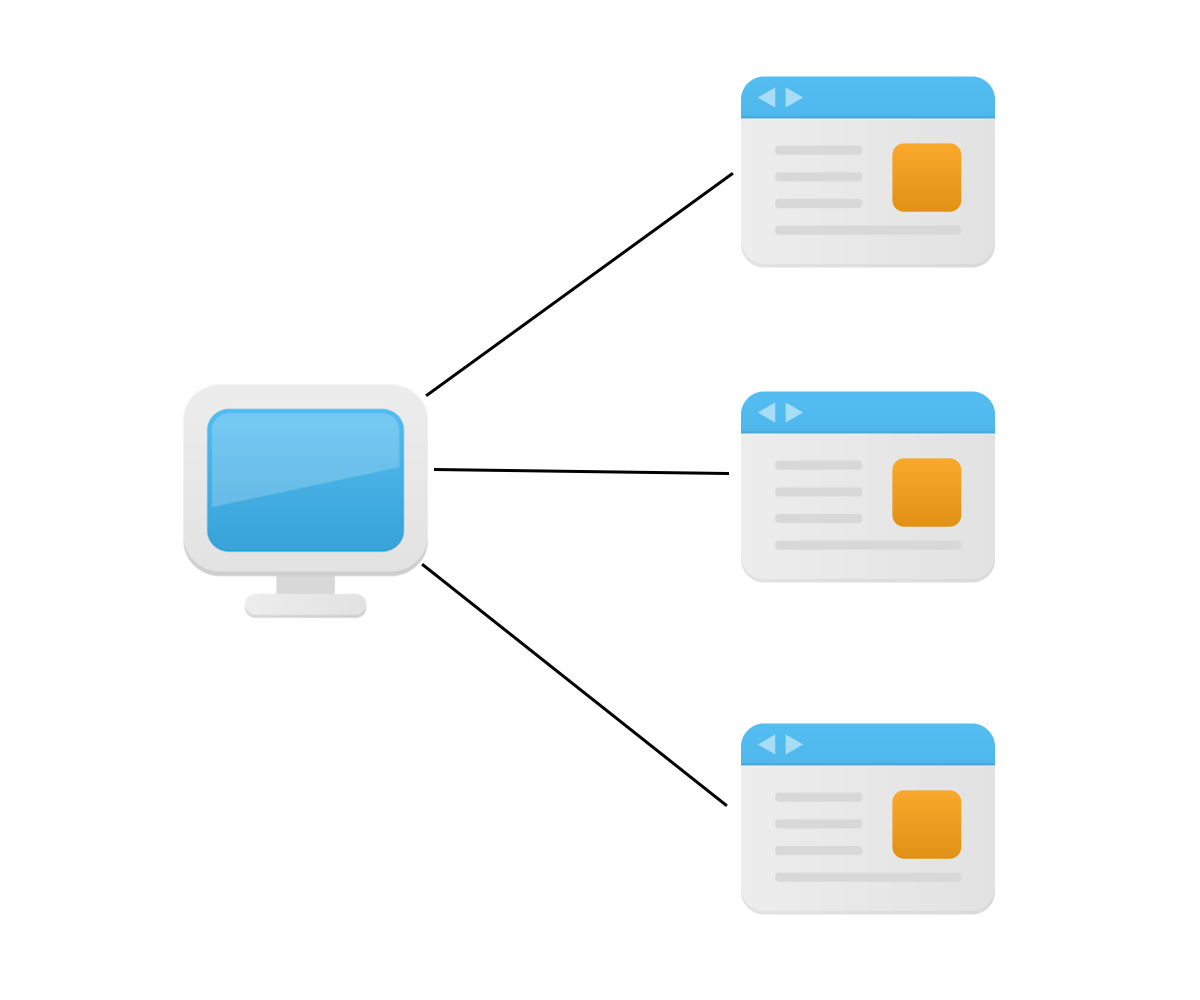
\includegraphics[width=6cm]{assets/siteweb}\newline

	\end{frame}

	\begin{frame}
		\frametitle{Présentation}

		Et une application web marche comme ça:
		\newline \newline

		\centering
		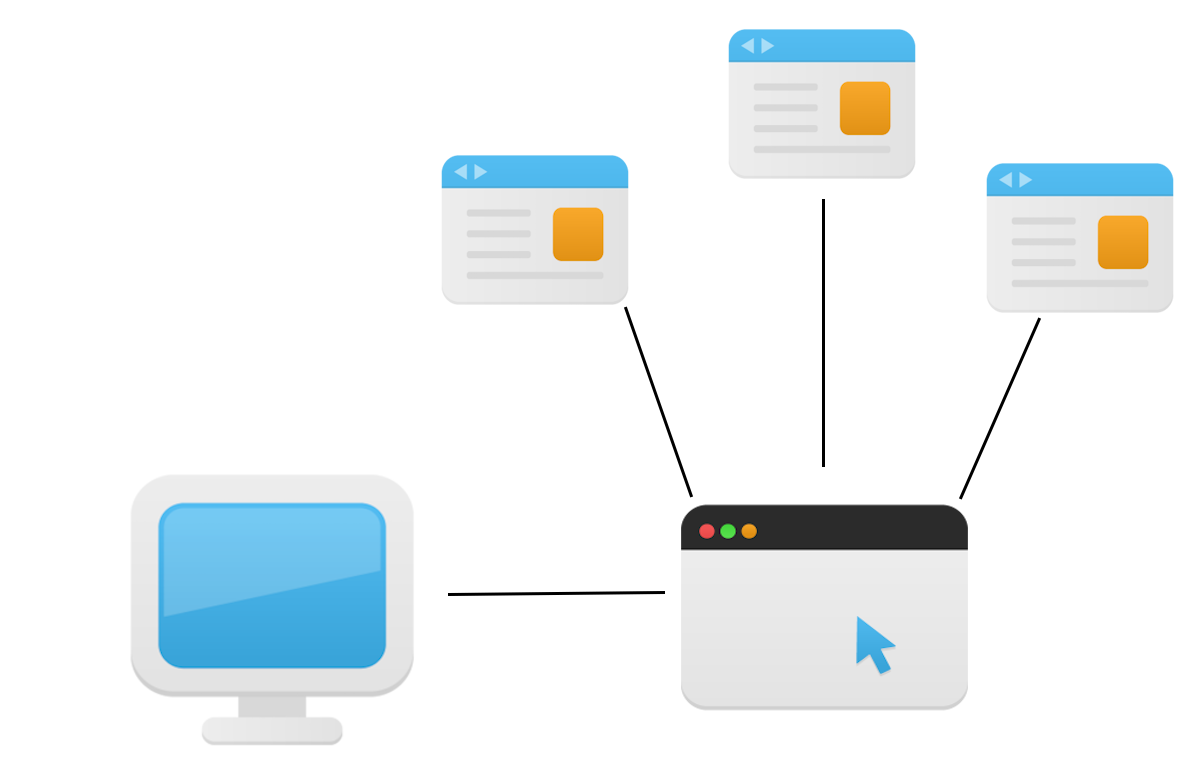
\includegraphics[width=8cm]{assets/appweb}\newline

	\end{frame}

	\begin{frame}
		\frametitle{Présentation}

		Resumé :
		\newline \newline
		le client doit faire une requête au serveur a chaque fois dans un site web \newline \newline
		alors que dans une application web, nous allons deleguer le travaille a JavaScript qui vas désactivé ou activé une parti du code html/css
		\newline \newline
		\begin{block}{Information}
			Cette méthode s'appel SPA (Single Page Application)
		\end{block}
	\end{frame}

	\begin{frame}
		\frametitle{Histoire}

		AngularJS n'est pas egal a Angular \newline \newline

		AngularJS à été créer par Google \newline \newline

		AngularJS avait comme architecture MVC \newline \newline

		AngularJS n'est plus maintenu depuis 2018 \newline \newline

		\begin{block}{MVC}
			Module Vue Controlleur (Comme Symfony)
		\end{block}

	\end{frame}

	\begin{frame}
		\frametitle{Histoire}

		Angular est un framework orienté composant \newline \newline

		Nous allons codé une multitude de petit composant qui formeront une application \newline \newline

		Un composant est une parti du site qui fonctionne de manière autonome sur une applicaiton

	\end{frame}














\end{document}